\documentclass{article}
\usepackage[utf8]{inputenc}
\usepackage[T1]{fontenc}
\usepackage[portuguese]{babel}

\usepackage{indentfirst}
\usepackage{makeidx}
\usepackage{stackengine}
\usepackage{amssymb}
\usepackage{amsthm}
\usepackage{hyperref}
\usepackage{color}
\usepackage{graphicx}

\usepackage{pdfpages}

\usepackage{booktabs}

\title{\bf{Aprendizagem Computacional - Trabalho Prático 3}\vspace{80mm}}
\author{\textbf{João Tiago Márcia do Nascimento Fernandes - 2011162899} \\
\textbf{Joaquim Pedro Bento Gonçalves Pratas Leitão - 2011150072}}
\makeindex

\begin{document}

\maketitle

\pagebreak

\renewcommand*\contentsname{Índice}
\tableofcontents

\pagebreak

\section{Introdução}

O presente trabalho foca-se na previsão e identificação de crises epiléticas, com base em informação de sinais cerebrais, recolhidos através da realização de um \emph{EEG} (ElectroEncefaloGrama).

Este exame recolhe dados relativos à atividade cerebral do paciente que o realiza, sendo possível extrair um conjunto de características que permite a identificação de momentos de ocorrência de crises epiléticas (denominadas situações \emph{ictais}) e de momentos nos quais o paciente não apresenta qualquer problema (denominadas situações \emph{não-ictais}).

O trabalho proposto visa a criação de uma aplicação em \emph{Matlab}, que analise os dados recolhidos após a realização de um \emph{EEG} a um paciente, e que identifique eventuais situações em que a atividade cerebral registada corresponde a uma situação de crise epilética.

Para proceder à identificação das situações \emph{ictais} e \emph{não-ictais}, a aplicação desenvolvida faz uso, na sua arquitetura interna, de redes neuronais, disponíveis na \emph{Neural Networks Toolbox} do próprio \emph{Matlab}.

Para avaliar o desempenho e performance da aplicação desenvolvida, procederemos à análise da sensibilidade e especificidade de cada rede neuronal implementada.

Estas métricas correspondem à percentagem de situações \emph{ictais} verdadeiras detetadas (\emph{sensibilidade}) e à percentagem de situações \emph{não-ictais} falsas detetadas (\emph{especificidade}), refletindo a performance da rede na classificação de um dado \emph{data set}: Uma elevada \emph{sensibilidade} implica uma boa deteção de situações \emph{ictais}, enquanto que uma elevada \emph{especificidade} implica uma boa deteção de casos \emph{não-ictais}.

Ambas as métricas constituem requisitos necessários para a sua utilização em ambiente clínico, e podem ser definidas da seguinte forma:

$$Sensibilidade \: = \frac{PositivosVerdadeiros}{PositivosVerdadeiros + FalsosNegativos}$$

$$Especificidade \: = \frac{NegativosVerdadeiros}{NegativosVerdadeiros + FalsosPositivos}$$

\vspace{.1cm}

No presente documento pretendemos apresentar de forma mais detalhada a aplicação desenvolvida, discutindo alguns detalhes da sua implementação e apresentando uma reflexão crítica sobre o seu desempenho e performance, nomeadamente da sua sensibilidade e especificidade.

\pagebreak

\section{Aplicação Desenvolvida}

Tal como referido anteriormente, a aplicação desenvolvida visa analisar os dados referentes a um \emph{EEG} de um paciente, identificando situações correspondentes a uma crise epilética.

Esta classificação pode ser realizada de duas formas distintas, que passamos a descrever.

Numa primeira abordagem, a que chamamos \emph{Classificação Individual}, é atribuído a cada elemento do conjunto de dados de entrada da aplicação uma de duas \emph{classes}, representadas por dois valores binários:

\begin{itemize}
\item Classe \emph{não-ictal}, correspondente a um estado normal do paciente (ausência de crises) e representada pelos valores \emph{1 0}

\item Classe \emph{ictal}, correspondente a uma situação de crise, e representada pelos valores \emph{0 1}
\end{itemize}

Na segunda abordagem, a que chamamos \emph{Classificação em Grupo}, o processo de classificação das entradas é realizado de forma semelhante, no entanto são considerados conjuntos de dados de entrada da aplicação, ao invés de cada elemento. Para este tipo de classificação podemos adotar duas métricas diferentes:

\begin{itemize}
\item Analisar o número de elementos consecutivos classificados individualmente como \emph{ictais}, comparando-o com um dado limiar. Neste caso, se, por exemplo, existirem pelo menos 10 elementos consecutivos classificados como \emph{ictais} então é detetada uma crise. Caso contrário nenhuma crise é detetada.

\item Adotar um sistema de classificação em janela deslizante, analisando o número de elementos classificados individualmente como \emph{ictias}, num dado universo restrito. Isto é, se pelo menos cinco dos últimos dez elementos foram classificados como \emph{ictais} então todos os elementos nesse conjunto são classificados como \emph{ictais}.
\end{itemize}

Optámos por adotar o segundo método de \emph{Classificação em Grupo}, considerando uma abordagem por janelas, uma vez que o primeiro método, na nossa opinião, não torna o classificador resistente a variações no tempo. Isto é, caso a saída obtida seja igual à esperada, mas com todos os elementos deslocados, por exemplo, em uma unidade este método irá considerar um número de classificações erradas muito maior do que numa abordagem por janelas.

De seguida apresentamos em maior detalhe a aplicação desenvolvida, salientando alguns dos seus aspetos mais importantes e relevantes.

\subsection{Graphical User Interface}

Para facilitar a interação do utilizador com a aplicação, foi-nos proposta a criação de uma interface gráfica onde são solicitadas ao utilizador todas as informações relevantes para a execução da aplicação, separando por completo a sua lógica interna com a especificação dos seus dados de entrada e outros parâmetros.

Assim, na interface gráfica desenvolvida são solicitadas ao utilizador várias informações que permitem a criação e treino das diferentes redes neuronais, nomeadamente:

\begin{itemize}
\item Tipo de rede neuronal a criar e treinar. Encontram-se disponíveis as redes \emph{Radial Basis Function}, \emph{Layer Recurrent Network}, \emph{FeedForward}, \emph{FeedForward Time Input Delay} e \emph{Distributed Time Delay}.

\item Função de Aprendizagem (ou Função de Treino) a utilizar na rede neuronal a criar (Se necessário). Encontram-se disponíveis as funções \emph{trainscg}, \emph{traingd} e \emph{trainrp}.

\item Função de Performance a utilizar no treino da rede neuronal (se necessário). Estão disponíveis as funções \emph{mse} (mean squared error) e \emph{sse} (sum squared error).

\item Função de Activação dos neurónios da rede neuronal a implementar (se necessário). Estão disponíveis as funções \emph{hardlim}, \emph{purelin}, \emph{logsig} e \emph{tansig}.

\item Tipo de Classificação a realizar (\emph{Individual} ou \emph{Em Grupo})

\item Ficheiro de dados a utilizar para treinar a rede criada

\item Ficheiro de dados a utilizar para testar a rede criada

\item Número de características dos pacientes a considerar

\item Outros aspetos, como objetivo do treino (\emph{Goal}), taxa de aprendizagem, etc
\end{itemize}

Para além disso, na interface desenvolvida, existe também uma secção onde são apresentados os resultados de cada teste realizado, nomeadamente a especificidade e sensibilidade da rede considera.

\begin{figure}[h]
  \centering
      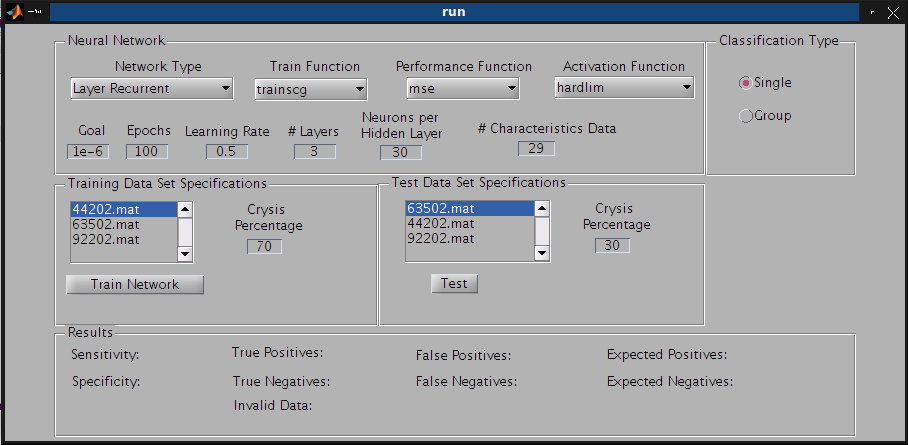
\includegraphics[scale=0.3]{Images/Aplication_GUI.png}
  \caption{Interface Gráfica implementada}
\end{figure}

\subsection{Redes Neuronais Implementadas}

Como já referimos anteriormente, na nossa aplicação implementámos cinco redes neuronais distintas: \emph{Radial Basis Function}, \emph{Layer Recurrent Network}, \emph{FeedForward}, \emph{FeedForward Time Input Delay} e \emph{Distributed Time Delay}.

Estas redes apresentam, naturalmente, características e propriedades distintas, sendo que umas se adequam mais ao trabalho que pretendemos realizar do que outras.

Por exemplo, considerando a rede \emph{Layer Recurrent}, esta rede permite a introdução de atrasos em algumas características, o que lhe permite aprender a prever qualquer saída dinâmica, tendo por base entradas passadas. Este processo é possível se forem considerados neurónios e atrasos suficientes na rede.

De facto, esta é uma propriedade que vai, de certa forma, ao encontro do funcionamento de um cérebro humano, que para além de ser um sistema dinâmico, possui também memória.

Na mesma linha de raciocínio, redes que suportam a introdução de atrasos em algumas das características que constituem os dados de entrada surgem, a uma primeira vista, como boas opções para simular o comportamento de um cérebro humano, realizando uma melhor identificação das situações correspondentes a crises epiléticas. Exemplos destas redes são a rede \emph{Distributed Time Delay} e a \emph{FeedForward Input Time Delay}.

Por seu turno, a rede \emph{FeedForward} também se apresenta como uma solução a considerar, dado o facto de permitir uma boa implementação de qualquer função de entradas e saídas arbitrárias, desde que considerados neurónios suficientes na(s) camada(s) escondida(s).

Por fim, é também necessário referir a rede \emph{Radial Basis Function}, bastante utilizada para aproximar funções e cujo treino passa nomeadamente pela adição de neurónios à camada escondida até que a rede atinja a performance (\emph{goal}) pretendida. Assim, embora possa ser necessário adicionar um elevado número de neurónios à camada escondida, acreditamos ser possível ter uma boa performance com esta rede.

\subsection{Treino das Redes}

Um dos principais aspetos do trabalho realizado, prende-se com o treino das redes neuronais, pois é ele que determina a boa (ou má) performance das redes implementadas.

Para o presente trabalho foram-nos fornecidos dados relativos a três pacientes, constituídos por um conjunto de características extraídas para cada elemento, e pela respetiva classe definida para cada elemento.

Uma vez que as situações em que os pacientes estão a sofrer de uma crise epilética são consideravelmente menos do que as situações em que o paciente não apresenta nenhum problema, a simples seleção de todos os elementos de um dos conjuntos fornecidos, ou de parte desses elementos, para realizar o treino da rede, sem qualquer cuidado na seleção dos elementos irá conduzir a dados de treino onde predominam situações \emph{não-ictais}.

Nesses casos, iremos verificar uma especialização da rede na identificação de situações \emph{não-ictais}, sem que faça uma classificação de casos \emph{ictais} igualmente fiável.

De facto, tal situação não é desejável, uma vez que o nosso principal objetivo passa pela identificação de casos \emph{ictais} com um grau de confiança mínimo, não a identificação de situações \emph{não-ictais}.

Assim, para evitar que as redes por nós treinadas se especializem em situações \emph{não-ictais}, na constituição dos casos de treino das diferentes redes neuronais, consideramos um dos ficheiros fornecidos, e para esse ficheiro selecionamos uma percentagem dos casos \emph{ictais} (essa percentagem é solicitada ao utilizador através da interface gráfica) que vamos incluir no nosso \emph{data set} de treino.

Em seguida, selecionamos um número igual de situações \emph{não-ictais}, preservando a ordem dos diferentes casos nos dados originais. Como o número de situações \emph{não-ictais} é bastante superior ao número de situações \emph{ictais}, ao selecionarmos um número de situações \emph{não-ictais} igual ao de situações \emph{ictais} temos, necessariamente de não incluir a maior parte das situações \emph{não-ictais}.

Para além disso, consideremos duas características observadas em dois momentos distintos do exame: Uma, observada num momento em que o paciente se encontra clinicamente estável (portanto numa situação \emph{não-ictal}); E outra, observada instantes antes da ocorrência de uma crise.

Embora ambas as situações sejam classificadas como \emph{não-ictais}, facilmente compreendemos que a segunda se encontra mais próxima de um estado \emph{ictal}, do que a primeira. Efetivamente, para evitar que as redes por nós treinadas classifiquem estas duas situações apresentadas com diferentes valores (atribuindo à primeira a classificação de \emph{não-ictal} e à segunda de \emph{ictal}), é necessário incluir, nos dados de treino das redes, uma porção de características que reflitam ambas as situações apresentadas, a par das situações \emph{ictais}.

Assim, para fazermos a seleção dos dados de treino das nossas redes, selecionamos aleatoriamente um conjunto de situações \emph{não-ictais} do conjunto de dados originais, preservando sempre a ordem de ambas as situações \emph{ictais} e \emph{não-ictais}, e assegurando a inclusão de exemplos referentes às duas situações apresentadas.

No processo de treino das redes recorremos ainda a diferentes funções de treino, disponíveis e implementadas pela \emph{Neural Network Toolbox} do \emph{Matlab}. As funções de treino disponíveis são a função \emph{traingd}, \emph{trainscg} e \emph{trainrp}.

Com exceção da rede \emph{RBF} (\emph{Radial Basis Function}) implementada, o treino das restantes redes neuronais é realizado com recurso à função \emph{train} da \emph{Neural Network Toolbox} do \emph{Matlab}. Uma vez que o treino das redes é uma operação complexa e exigente em termos computacionais, tendo em conta o tipo de redes criadas e a dimensão dos dados para proceder ao treino das redes, estas foram treinadas com aceleração gráfica, disponível nas versões mais recentes do \emph{Matlab}. Para tal, basta adicionar os parâmetros \emph{'useGPU', 'yes'} aquando da chamada da função \emph{train}: \emph{train(network, P, T, 'useGPU', 'yes')}.

Para a rede \emph{RBF}, o \emph{Matlab} realiza o seu treino aquando da criação da rede, não sendo necessária a invocação da função \emph{train}.

\subsection{Teste das Redes}

Uma vez completo o treino de uma rede neuronal, esta pode ser testada, de forma a verificar o seu bom, ou mau, funcionamento. Para isso, criámos um conjunto de dados de teste, baseados nos três \emph{data sets} inicialmente fornecidos.

O processo de criação dos dados de teste é semelhante ao utilizado na constituição dos dados de treino das redes neuronais:

É solicitado ao utilizador que indique o ficheiro (de entre os três ficheiros fornecidos) de onde serão extraídos os dados de teste, e qual a percentagem de situações \emph{ictais} a incluir. Em seguida, o ficheiro escolhido é analisado, e são considerados todos os dados nele presentes, a partir do final do ficheiro, até que o número de situações \emph{ictais} incluídas seja igual à percentagem especificada.

Por outras palavras, se o utilizador especifica que pretende incluir $25\%$ das situações \emph{ictais} nos dados de treino, e se todas as situações \emph{ictais} identificadas nesse \emph{data set} se encontram nas posições $10-20$, $40-50$, $60-70$ e $80-100$, então o nosso \emph{data set} de treino será constituído por todos os elementos do ficheiro, desde a posição $60$ até ao final do ficheiro.

Uma vez que aquando da realização dos testes na rede esta já se encontra treinada, é irrelevante considerarmos nos \emph{data sets} de teste situações \emph{ictais} na mesma ordem de grandeza do que situações \emph{não-ictais}, pois apenas estamos a executar a rede para um conjunto de dados, sem que este afete de forma alguma o funcionamento da rede em situações futuras.

\subsection{Implementação em Matlab}

A aplicação foi por nós desenvolvida e programa quase na sua totalidade, com a exceção do código relativo à interface gráfica. Esta foi desenhada por nós através da interface \emph{guide} do \emph{Matlab}, tendo o seu código sido gerado pelo \emph{Matlab}.

De qualquer forma, toda a lógica interna da aplicação, comunicação da informação recolhida pela interface gráfica para outras estruturas, etc, foi por nós completamente desenvolvida.

\subsubsection{run.m}

Este é o principal ficheiro da aplicação e que permite a sua execução. É nele que se encontra todo o código gerado, relativo à interface gráfica, mas também onde todas as principais funcionalidades da aplicação (criação das redes neuronais e respetivo treino e classificação dos dados de teste) são invocadas.

\subsubsection{createNetwork.m}

No ficheiro \emph{createNetwork.m} encontramos a função \emph{createNetwork}, responsável pela criação da rede neuronal que irá realizar a identificação das  situações \emph{ictais} nos dados considerados e fornecidos à aplicação. 

Esta rede é criada de acordo com algumas características pré-definidas, e outras escolhidas pelo utilizador, como é o caso das funções de ativação e de treino.

Após a sua criação, a rede será treinada com um conjunto de dados previamente criado de acordo com as especificações fornecidas pelo utilizador. Este treino não é realizado neste ficheiro, mas sim no principal ficheiro desenvolvido para a aplicação, \emph{run.m}.

\subsubsection{prepareDataSets.m}

Neste ficheiro encontramos a função \emph{prepareDataSets}, responsável pela criação dos \emph{data sets} de treino e e de teste, bem como dos respetivos resultados esperados (quer para os dados de treino, quer para os dados de teste). Para além disso, neste ficheiro é ainda invocado o procedimento responsável pela seleção das principais características registadas, para o paciente em questão, que abordaremos em maior detalhe mais à frente nesta secção.

Tal como referimos brevemente numa secção anterior do presente documento, as abordagens seguidas para a criação dos conjuntos de dados de treino e de teste têm pontos em comum, não sendo, no entanto, completamente iguais.

Uma vez que, nos ficheiros fornecidos, o número de situações \emph{não-ictais} é bastante superior à quantidade de classificações \emph{ictais}, se simplesmente considerarmos para o nosso \emph{data set} de treino uma percentagem dos dados fornecidos, sem nos preocuparmos com a distribuição de situações \emph{não-ictais} e \emph{ictais}, então será altamente provável que as nossas redes sejam treinadas com mais casos \emph{não-ictais} do que com \emph{ictais}, resultando numa especialização da mesma na deteção de situações \emph{não-ictais}.

Efetivamente, tal situação corresponde ao oposto do desejável, tendo em conta que o nosso objetivo principal passa pela identificação de casos \emph{ictais}, com um grau de confiança mínimo.

Assim, para os dados de treino das redes neuronais criadas são consideradas situações \emph{ictais} e \emph{não-ictias} em igual número e de acordo com uma percentagem das situações \emph{ictais} totais do ficheiro a considerar, definida pelo utilizador. Nesta seleção, tal como referido anteriormente, é preservada a posição relativa das situações \emph{ictais} e \emph{não-ictais} consideradas, e assegurando a inclusão de exemplos referentes Às duas situações \emph{não-ictais} apresentadas.

No que respeita aos dados de teste, também criados neste ficheiro, não é necessária qualquer preocupação em relação ao número de situações \emph{ictais} e \emph{não-ictais}, uma vez que pretendemos utilizar estes dados em redes já treinadas, pelo que a sua execução em nada alterará o comportamento futuro da rede.

Assim, os dados de treino são construídos partindo do final de um ficheiro de dados previamente selecionado, incluindo todos os dados (correspondentes a casos \emph{ictais} e \emph{não-ictais}) até que o número de situações \emph{ictais} seja igual a um valor definido pelo utilizador.

\subsubsection{processCharacteristics.m}

Neste ficheiro podemos encontrar o procedimento responsável pela seleção das principais características registadas, para o paciente em questão.

Esta seleção é feita com base numa análise da correlação entre as diferentes características registadas e a classificação esperada para cada conjunto, selecionando as características que apresentam valores de correlação mais elevados, e em número igual ao especificado pelo utilizador na interface gráfica.

Com este procedimento pretendemos eliminar características redundantes dos nossos ficheiros de dados. Embora seja de prever que esta eliminação em nada altere a aprendizagem da rede (ou, em caso de alteração, que esta seja bastante ténue), é expectável uma melhoria no seu tempo de treino proporcional ao número de características redundantes removidas.

\subsubsection{interpretResults.m}

É neste ficheiro que se encontra a função \emph{interpretResults}, onde é realizado o processamento da classificação executada pela rede neuronal treinada, nas situações em que o tipo de classificação escolhido é a \emph{Classificação Individual}.

Este processamento consiste simplesmente em percorrer os resultados obtidos na execução da rede neuronal para o caso de teste fornecido, comparando-os elemento a elemento com os resultados esperados para esse caso de teste. Assim, é registado o número de situações em que a classificação da rede se apresenta correta (distinguindo-se entre classificações de situações \emph{ictais} e \emph{não-ictais}), bem como situações em que a classificação da rede está incorreta (também distinguindo-se entre ituações \emph{ictais} e \emph{não-ictais}).

Para além disso, são também registados o número de classificações positivas e negativas, isto é, de situações \emph{ictais} e \emph{não-ictais}, presentes nos dados fornecidos à rede, e que num cenário de classificação perfeita corresponderiam ao número de situações \emph{ictais} e \emph{não-ictais} registadas.

Uma vez que a classificação realizada pela rede nem sempre é clara, podem existir situações para as quais a rede não convergiu, não sendo possível distinguir de forma clara para uma dada situação (ou conjunto de situações) qual a classe atribuída pela rede. Essas situações são também registadas nesta função, sendo posteriormente reportadas como classificações inválidas.

\subsubsection{interpretGroupResults.m}

O ficheiro \emph{interpretGroupResults.m} é responsável por uma importante parte da lógica subjacente à \emph{Classificação em Grupo} realizada pela aplicação.

Neste ficheiro, a abordagem seguida é em tudo semelhante ao realizado no caso da \emph{Classificação Individual}: Possuindo os resultados esperados para o teste realizado, basta percorrer os dados obtidos como resultado da classificação da rede neuronal, registando as situações em que os dois conjuntos de dados (dados obtidos e esperados) são idênticos (verdadeiros positivos e verdadeiros negativos), bem como situações onde as classificações diferem (falsos positivos e falsos negativos), ou então não são possíveis (classificações inválidas).

\subsection{Execução}

Para executar a aplicação o utilizador simplesmente necessita de executar o ficheiro \emph{run.m}, sendo imediatamente exibida a interface gráfica desenvolvida.

A partir desse momento, o utilizador poderá escolher a rede a criar e a treinar, definindo algumas das suas propriedades e do seu treino, nomeadamente a escolha do ficheiro de dados a utilizar como fonte para a criação dos dados de treino e para posterior teste da rede treinada. É também possível selecionar o tipo de classificação a realizar, e o número de características a considerar.

Uma vez definidos todos os parâmetros pretendidos pelo utilizador, basta clicar na opção \emph{Train Network}, para proceder ao treino da rede, ou na opção \emph{Test}, para proceder à execução da rede para os dados de teste especificados.

Queremos também salientar a possibilidade de seleção a opção \emph{Test} sem, previamente, ter sido treinada nenhuma rede. Nesse caso, será criada e treinada uma rede de acordo com as especificações para esta definidas na interface. Caso o utilizador não tenha definido nenhuma configuração, será utilizada uma por defeito.

Uma vez finda a execução da rede para os dados de treino selecionados, os resultados dessa execução poderão ser visualizados no painel \emph{Results}, estando disponível a \emph{sensibilidade} e \emph{especificidade} registadas, bem como os dados que permitiram calcular esses valores (verdadeiros positivos e negativos, e falsos positivos e negativos). É ainda apresentado o número de classificações inválidas registadas. 

\pagebreak

\section{Treino e Testes da Aplicação}
\label{sec:train_tests}

Após o desenvolvimento inicial da aplicação procedemos ao treino e teste das diferentes redes implementadas, a fim de aferir o seu correto, ou incorreto, funcionamento e da sua adequação às nossas previsões iniciais para a performance de cada rede.

\subsection{Testes Iniciais}

\subsubsection{Descrição}

Numa fase inicial dos testes realizados procedemos ao treino de todas as redes neuronais implementadas, para uma vasta gama de combinações possíveis das propriedades das redes consideradas, e para os dois tipos de classificação disponíveis. Assim, inicialmente treinámos as redes com as seguintes propriedades: 

\begin{itemize}
\item Redes treinadas com os dados dos ficheiros \emph{44202.mat} e \emph{63502.mat}

\item Percentagem de situações \emph{ictais} consideradas nos casos de treino de $30\%$, $50\%$ e $70\%$

\item Objetivo do treino com o valor de $10^{-6}$, com exceção da rede \emph{Radial Basis Function}, onde o valor considerado foi de $10^{-2}$

\item Número de épocas de treino máximo de $1000$

\item Número de \emph{validation checks} necessários para terminar o treino igual a metade do número máximo de épocas de treino, ou seja $500$

\item Ritmo de aprendizagem de $0.5$

\item Rede constituída por $1$ camada escondida

\item Número de neurónios por cada camada escondida tomando os valores $3$, $log_{2} (29) = 5$ e $29$ 

\item Funções de ativação consideradas: \emph{hardlim}, \emph{purelin}, \emph{logsig} e \emph{tansig}

\item Funções de treino consideradas: \emph{trainscg}, \emph{traingd} e \emph{trainrp}

\item Funções de performance consideradas: \emph{sse} e \emph{mse}
\end{itemize}

Em anexo a este documento encontra-se uma lista detalhada dos resultados obtidos em cada teste realizado, que poderá ser consultada pelo leitor.

Na lista apresentada optámos por não incluir os resultados relativos aos testes para as redes treinadas com a função \emph{sum squared error} como função de performance, uma vez que as redes treinadas com esta função obtiveram valores de performance registados pela \emph{Neural Network Toolbox} muito superiores aos registados para as redes treinadas com a função de performance \emph{mean squared error}\footnote{Neste caso, quanto maior for o valor registado para a performance de uma rede pior será o seu desempenho}.

Por essa razão, ao procedermos à análise dos resultados obtidos não iremos incidir sobre as redes treinadas com a função de performance \emph{sse}, uma vez que os seus resultados não apresentam grandes diferenças, nem se destacam por realizarem uma classificação aceitável.

De seguida iremos proceder a uma análise mais detalhada sobre os resultados obtidos, começando por incidir nos testes realizados para a \emph{Classificação Individual}, passando de seguida para a \emph{Classificação em Grupo}.

\subsubsection{Análise dos Resultados Obtidos para Classificação Individual}

Antes de procedermos à análise individual de cada rede implementada e testada pretendemos proceder a uma descrição geral do comportamento das redes neste conjunto de testes.

De uma forma geral, as diferentes redes testadas apresentaram, para pelo menos uma constituição (número de neurónios na camada escondida, objetivo do treino, função de treino, ativação e performance, etc) valores de \emph{especificidade} e \emph{sensibilidade} que consideramos aceitáveis para o trabalho em questão, isto é, iguais ou superiores a $0.7$.

De facto, para utilização da aplicação numa situação real consideramos que um valor de $0.7$ poderá não ser aceitável, no entanto tendo em conta o objetivo do trabalho, o seu contexto e os dados utilizados, $0.7$ parece-nos um valor aceitável.

Outro fenómeno também comum a praticamente todas as redes (com exceção da rede \emph{Radial Basis Function}), tem que ver com o número de classificações inválidas detetadas. Nunca foi registado o valor 0 (novamente, exceto para a rede \emph{Radial Basis Function}), e nas situações em que foram registados valores mais elevados verificou-se uma grande variação dos valores de \emph{especificidade} e \emph{sensibilidade} registados, prevalecendo a \emph{especificidade} das redes em questão.

Concentrando-nos na rede \emph{Radial Basis Function}, podemos verificar que esta obteve muitos dos melhores registos para estes testes, com valores de \emph{especificidade} e \emph{sensibilidade} no intervalo $[0.8,0.9]$. Efetivamente, esta rede registou piores resultados quando limitada a $29$ neurónios.

De facto, seria de esperar que possuindo um número de neurónios igual ao número de características consideradas no treino, a rede realizasse melhores classificações, no entanto tal não se verificou. Não obstante, tal resultado pode também dever-se ao \emph{goal} com que esta rede foi treinado que, por ser bastante reduzido, (apenas $0.02$) irá certamente afetar a performance da rede.

Analisando os resultados obtidos para a rede \emph{FeedForward} podemos facilmente constatar que a rede tem uma maior \emph{especificidade} do que \emph{sensibilidade}, uma vez que a primeira toma valores no intervalo $[0.8,0.9]$ e a segunda no intervalo $[0.6,0.7]$. Para além disso, foram registados melhores resultados para as redes treinadas com as funções \emph{trainrp} e \emph{trainscg}.

Ao treinar e testar a rede com dados do ficheiro \emph{63502.mat} verificámos uma melhoria nos valores de \emph{especificidade} registados, que passaram a rondar o $0.9$. No entanto, a \emph{sensibilidade} desceu bruscamente, ocorrendo situações onde se registaram valores inferiores a $0.5$.

No que diz respeito à rede \emph{Layer Recurrent} a função de treino \emph{trainrp} foi a que registou piores valores de \emph{especificidade} e \emph{sensibilidade}. Nos restantes casos, os valores de \emph{sensibilidade} também não foram demasiado elevados, variando desde os $0.4$ até aos $0.7$. Para a \emph{especificidade}, já foram registados valores mais elevados, pertencentes ao intervalo $[0.7,0.9]$.

No treino desta rede com dados do ficheiro \emph{63502.mat}, considerando $3$ neurónios e testes com $30\%$ das situações \emph{ictais} com a função \emph{trainrp} verificámos a ocorrência de valores elevados para a \emph{especificidade}, mas bastante baixos para a \emph{sensibilidade}. Mais ainda, registou-se uma situação, para o mesmo ficheiro mas com testes com $70\%$ das situações \emph{ictais}, onde a \emph{especificidade} toma o valor $1$ e a \emph{sensibilidade} é nula.

Por fim, as redes \emph{Distributed Time Delay} e \emph{FeedForward Input Time Delay} obtiveram resultados muito próximos, registando-se muitas oscilações entre os valores de \emph{especificidade} e \emph{sensibilidade} para o mesmo teste. Os melhores resultados registados para estas redes foram conseguidos utilizando a função \emph{trainscg} como função de treino.

\subsubsection{Análise dos Resultados Obtidos para Classificação em Grupo}

Após a análise dos resultados obtidos para a \emph{Classificação Individual}, o cenário observado para a \emph{Classificação em Grupo} não é muito diferente: De uma forma geral as redes mostraram o mesmo comportamento que nos testes anteriores, tendo-se registado algumas variações face ao observado anteriormente, que queremos destacar:

Em primeiro lugar, nos testes agora realizados as variações, para a mesma situação, de valores muito elevados de \emph{especificidade} e muito reduzidos de \emph{sensibilidade} (e vice-versa) não só estão presentes como são mais regulares e evidentes: Por exemplo, nas redes \emph{Layer Recurrent}, \emph{Distributed Time Delay} e \emph{FeedForward Input Time Delay}, registámos várias situações com \emph{especificidades} de $1$, e \emph{sensibilidades} de $0$, e vice-versa.

Em segundo lugar, verificámos a existência de muito menos classificações inválidas, algo só igualado na \emph{Classificação Individual} pela rede \emph{Radial Basis Function}, que não realizou qualquer classificação inválida.

\subsection{Redução da Dimensionalidade}

\subsubsection{Descrição}

Com base nos resultados e análises realizadas anteriormente, concluímos que as redes capazes de realizar uma melhor classificação e identificação dos estados \emph{ictais} são as seguintes:

\begin{itemize}
\item Rede \emph{Radial Basis Function} com $3$ e $5$ neurónios

\item Rede \emph{FeedForward} com $3$, $5$ e $29$ neurónios, utilizando as funções de treino \emph{trainrp} e \emph{trainscg}

\item Rede \emph{Layer Recurrent} com $3$, $5$ e $29$ neurónios, utilizando as funções de treino \emph{trainrp} e \emph{trainscg}

\item Rede \emph{Distributed Time Delay}, com $3$, $5$ e $29$ neurónios, utilizando a função de treino \emph{trainscg}
\end{itemize}

Assim, nesta secção, pretendemos avaliar a prestação destas redes, quando treinadas com conjuntos de dados semelhantes aos utilizados, mas removendo algumas características mais redundantes.

Embora não sejam de esperar melhoras muito significativas na \emph{especificidade} e \emph{sensibilidade} das redes, ao remover características redundantes dos \emph{data sets} esperamos reduzir significativamente o tempo de treino das redes (idealmente até valores onde já não fosse necessário recorrer a processamento gráfico como forma de acelerar o treino das redes).

\subsubsection{Testes}

Nos testes realizados, procedemos a reduções de dimensionalidade dos dados de treino e de teste, considerando apenas as $5$ e $15$ características com maior correlação com a classificação final.

Para determinarmos quais as características a considerar, recorremos à função \emph{corrcoef} do \emph{Matlab}, obtendo, para cada ficheiro utilizado, as correlações de cada característica com a classificação final esperada.

Uma vez obtidos estes valores, restou-nos proceder à sua ordenação, escolhendo por fim as características com maior valor de correlação, nas quantidades referidas.

Uma vez determinadas as características a considerar, determinámos os dados de treino e teste das redes (considerando apenas estas características), procedendo de seguida ao treino e teste das redes referidas anteriormente.

Os resultados dos testes realizados podem ser consultados no final do presente documento, na secção destinada aos anexos, após a apresentação dos resultados dos testes iniciais.

De uma forma geral, para a \emph{Classificação Individual e em Grupo} não verificamos diferenças significativas, quando treinamos as redes com um menor número de características:

Na \emph{Classificação Individual} continuamos a presenciar algumas variações nos valores de \emph{sensibilidade} e \emph{especificidade} para o mesmo teste, mantendo-se também a rede \emph{Radial Basis Function} como a única rede a não realizar \emph{classificações inválidas}.

Já na \emph{Classificação em Grupo}, o número de testes onde se detetam \emph{classificações inválidas} é bastante reduzido, sendo que quando estas são detetadas o seu número é bastante elevado. Para além disso, também se verificam algumas variações nos valores de \emph{sensibilidade} e \emph{especificidade} para o mesmo teste.

Não obstante, à luz do que esperávamos (e que também referimos anteriormente), constatámos que, ao considerarmos um número de características inferior, o tempo necessário para treinar as diferentes redes neuronais diminuiu consideravelmente, nomeadamente quando apenas considerámos as $5$ características mais importantes.

\pagebreak

\section{Conclusões}

Após uma análise crítica dos testes e respetivos resultados obtidos, existem alguns pontos aos quais pretendemos dar destaque.

Em primeiro lugar, em ambos os conjuntos de testes realizados, redes (e respetivas configurações) que apresentaram melhores resultados foram as seguintes:

\begin{itemize}
\item Rede \emph{Radial Basis Function} com $3$ e $5$ neurónios

\item Rede \emph{FeedForward} com $3$, $5$ e $29$ neurónios, utilizando as funções de treino \emph{trainrp} e \emph{trainscg}

\item Rede \emph{Layer Recurrent} com $3$, $5$ e $29$ neurónios, utilizando as funções de treino \emph{trainrp} e \emph{trainscg}

\item Rede \emph{Distributed Time Delay}, com $3$, $5$ e $29$ neurónios, utilizando a função de treino \emph{trainscg}
\end{itemize}

Da mesma forma, dos dois ficheiros com os quais realizámos os testes, foi com os dados do ficheiro \emph{44020.mat} que foram registados os melhores resultados, superando assim o ficheiro \emph{63502.mat}.

Isto poderá ser devido ao facto de, o paciente cujos dados se encontram no ficheiro \emph{44020.mat} possuir uma atividade cerebral mais favorável ao diagnóstico de situações \emph{ictais}, recorrendo à abordagem por nós adotada, com os tipos de rede escolhidos. Embora consideremos que não dispomos dos conhecimentos médicos necessários para produzir esta afirmação com um grau de confiança bastante elevado, esta parece-nos ser uma justificação válida.

Relativamente às funções de treino estudadas, a função \emph{trainscg} provou ser a melhor, uma vez que praticamente todas as redes nas quais esta foi utilizada obtiveram melhores resultados, quando comparados com as restantes, do mesmo tipo.

Ao diminuirmos as características com que procedíamos aos treinos e teste da rede os resultados que obtivemos confirmaram as nossas expetativas, uma vez que não verificámos variações significativas na \emph{sensibilidade} e \emph{especificidade} das redes testadas.

De facto, ao considerarmos apenas as características que têm uma maior contribuição para a saída desejada é expetável que a aprendizagem realizada pela rede não saia demasiado prejudicada. Tal situação só será contemplada se o número de características consideradas for demasiado reduzido, excluindo características com bastante influência na determinação no valor obtido à saída da rede neuronal.

Efetivamente, para o número de características consideradas verificámos que a aprendizagem não sofria penalizações significativas, mesmo considerando apenas as $5$ características mais influentes para o resultado final.

Mais ainda, ao realizarmos o treino das redes com um menor número de características, tal como esperado, observamos que o tempo de treino das redes baixou consideravelmente. Com efeito, uma vez que o número de características a considerar é menor, o número de passos a realizar em cada iteração do treino é menor, o que reduz o tempo de treino.

Mais ainda, procedendo à eliminação das características mais ambíguas, é de esperar que a rede apresente uma maior e mais rápida convergência, melhorando também a sua performance e o seu tempo de treino, o que foi por nós verificado.

\pagebreak

\section{Anexos}

Nas páginas seguintes apresentamos resultados obtidos para todos os testes realizados.

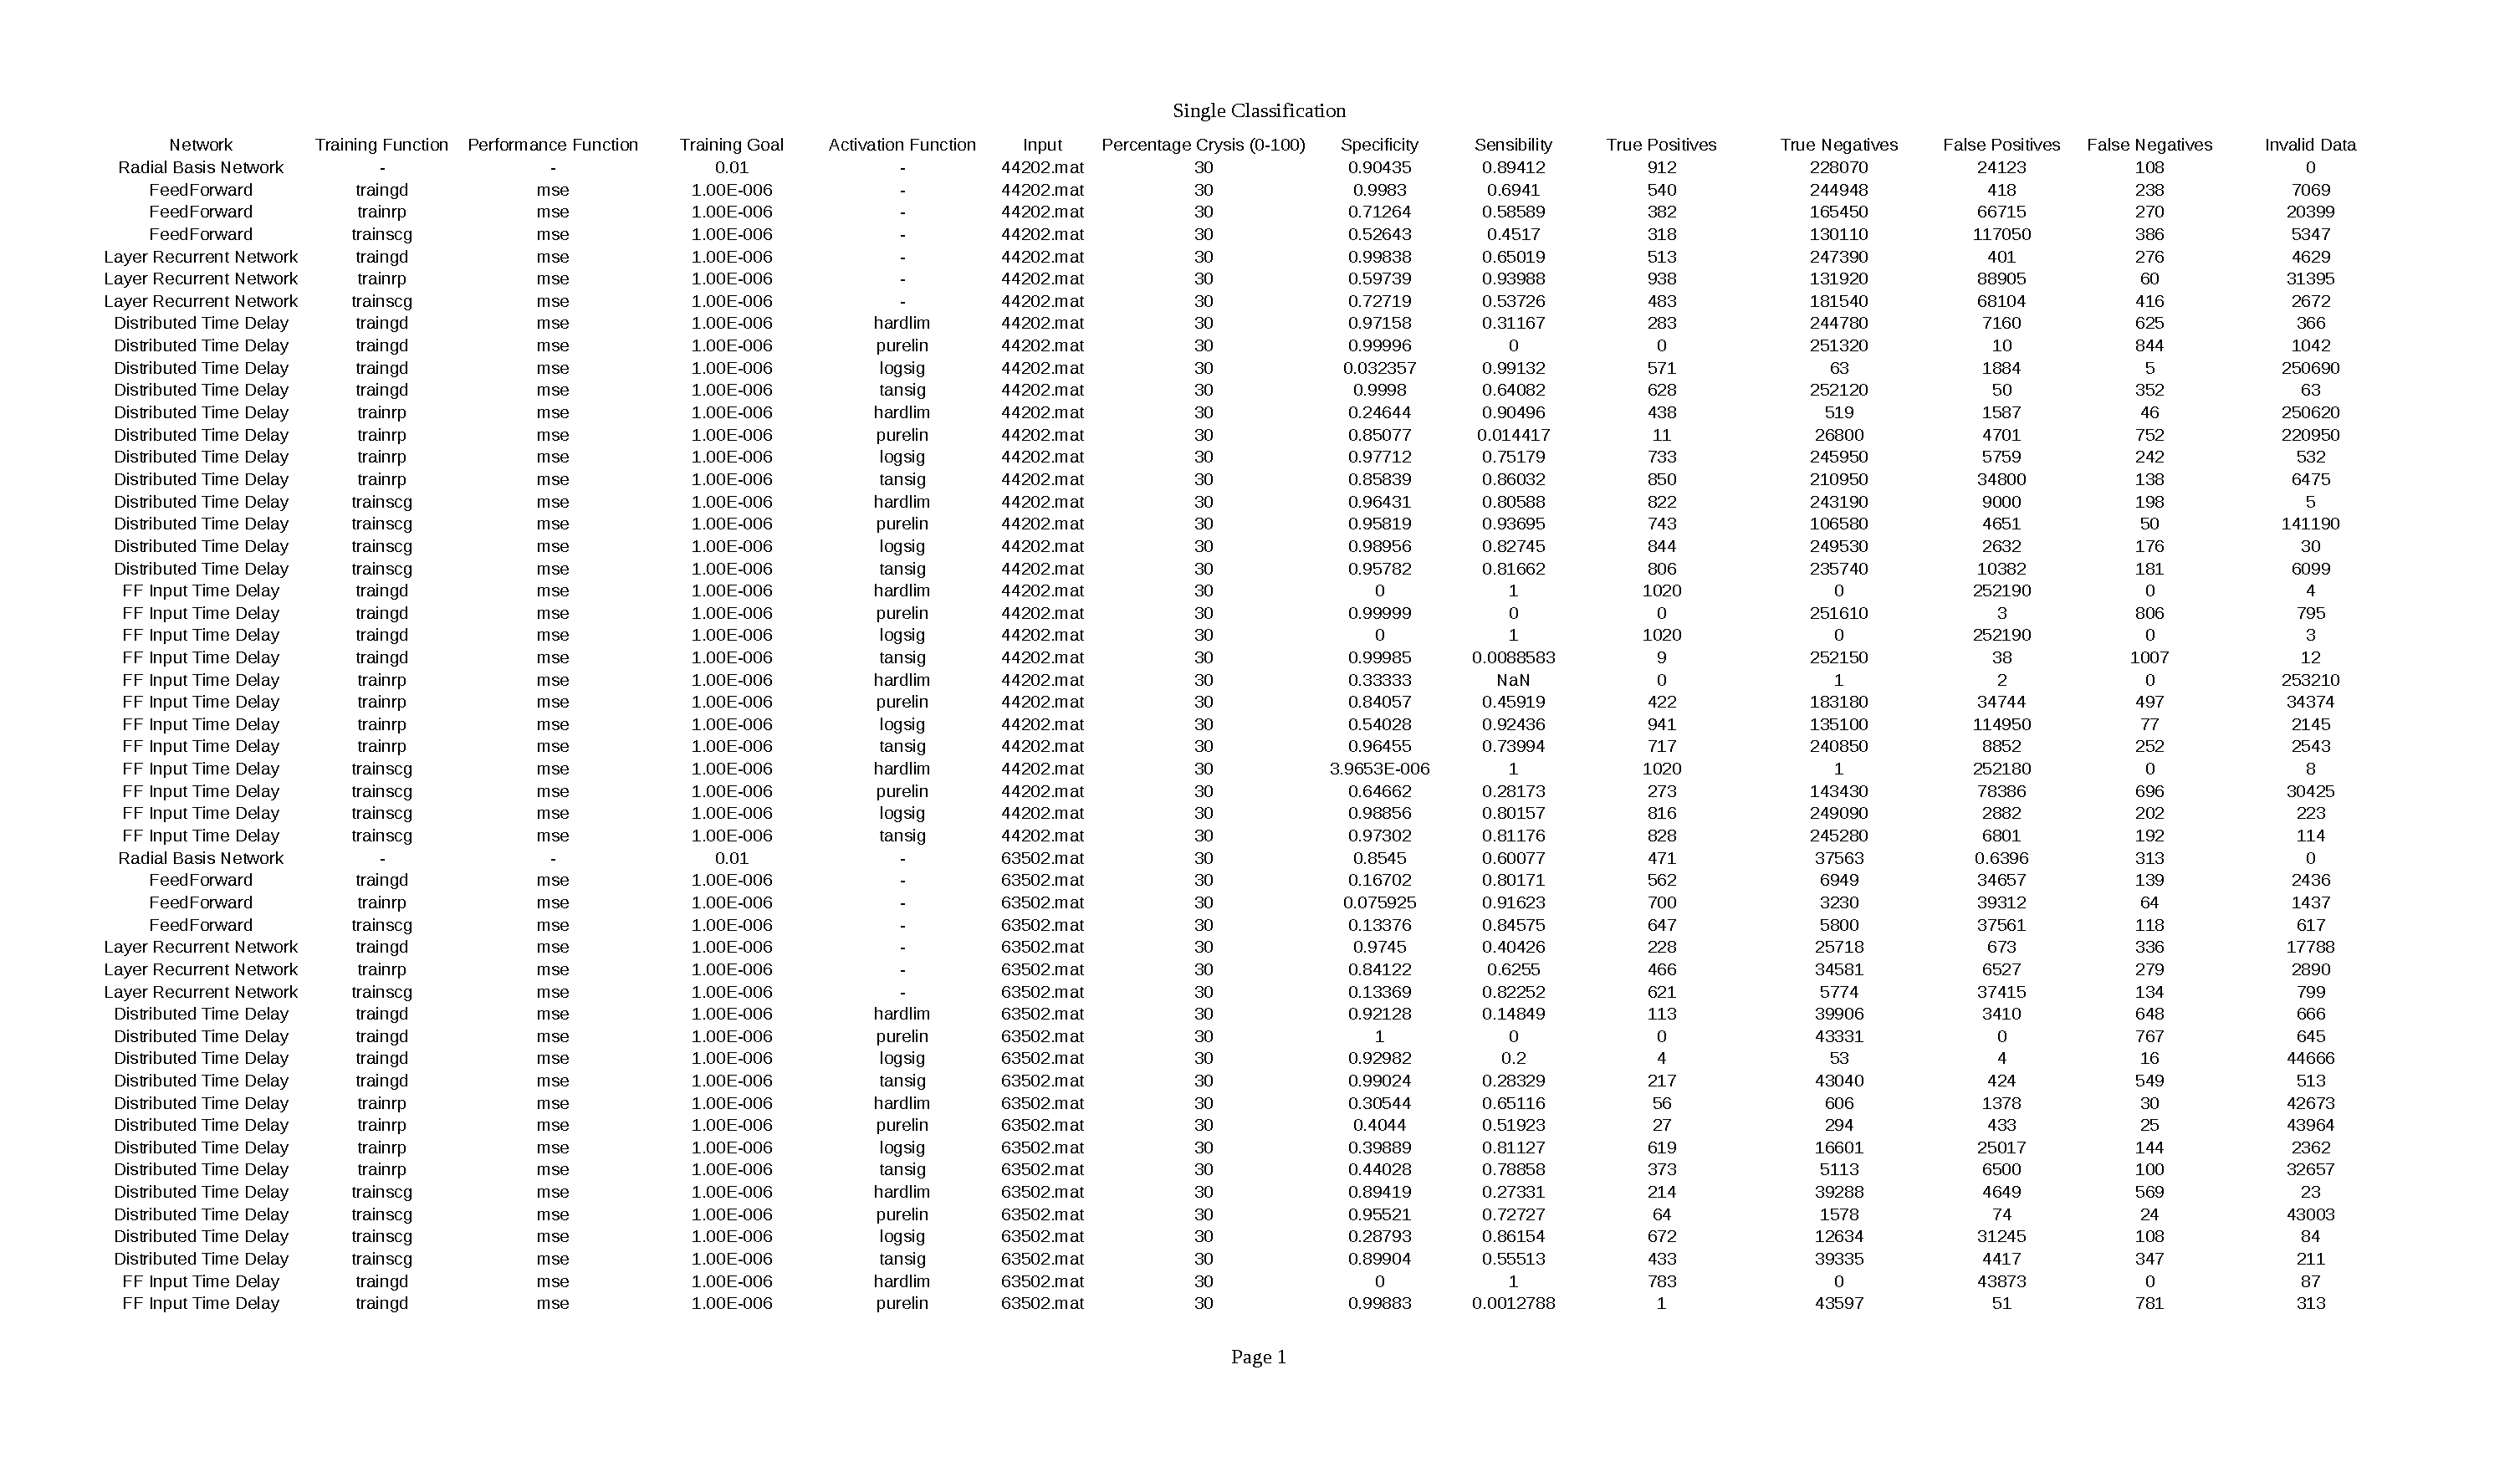
\includepdf[pages={1-32}, landscape=true]{Images/Results.pdf}

\end{document}